\documentclass[hidelinks]{ctexart}

\usepackage{van-de-la-illinoise}
\usepackage{cmbright}
\usepackage{nccmath}
\usepackage[paperheight=297mm,paperwidth=240mm,top=.2in,left=.1in,right=.1in,bottom=.2in, landscape]{geometry}
\usepackage{tensor}
\usepackage{stackengine}

\definecolor{graybg}{RGB}{228,235,243}
\definecolor{titlepurple}{RGB}{150,131,104}
\definecolor{shadegray}{RGB}{102,119,136}
\definecolor{itemgray}{RGB}{163,149,128}
\definecolor{mathnormalblack}{RGB}{0,0,0}
\pagecolor{graybg}

\setCJKmainfont{STHeitiSC-Light}
\setmainfont{Arial}

\usepackage{multicol}
\setlength{\columnsep}{.1in}

\newcommand{\raisedrule}[2][0em]{\qquad}
%\leaders\hbox{\rule[#1]{1pt}{#2}}\hfill}
\newcommand{\wdiv}{\,·\,}

\setlength{\parindent}{0pt}

\setCJKfamilyfont{pfsc}{STYuanti-SC-Regular}
\newcommand{\titlefont}{\CJKfamily{ttt}}
\setCJKfamilyfont{ttt}{STFangsong}
\newcommand{\mathtextfont}{\CJKfamily{ttt}}
\def\bili#1#2{#2}

\newdimen\indexlen
\def\newheader#1{%
\def\probindex{#1}
\setlength\indexlen{\widthof{\Large\color{titlepurple} #1\qquad}}
\vspace{1em}
{\Large\color{titlepurple} #1\qquad}
\raisebox{.5em}{\tikz \fill[titlepurple,opacity=.2,path fading=east] (0,0.05em) rectangle (\dimexpr\linewidth-\indexlen\relax,0em);}
}
\def\mathitem#1{\text{\color{itemgray}#1}}
\def\mathcomment#1{\text{\color{lightgray}\quad \texttt{\#}\kern-0pt#1}}
\def\mathheadcomment#1{\text{\color{lightgray}\texttt{\#}\kern-0pt#1}}
\def\midbreak{\smash{\raisebox{1.5em}{\smash{\tikz \path[opacity=.2,left color=white,right color=white,middle color=black] (0,0.05em) rectangle (\linewidth,0em);}}}
\vspace{-4em}}
\newtcolorbox{cheatresume}{enhanced, arc=.5pt, left=.5em, frame hidden, boxrule=0pt, colback=white, fuzzy halo=.05pt with lightgray, shadow={.4pt}{-.4pt}{0pt}{fill=shadegray,opacity=0.3}}

\usetikzlibrary{arrows.meta}
\usetikzlibrary{positioning}

\begin{document}

\begin{multicols*}{3}[\centerline{\titlefont 原子の波動関数及び微細構造、Zeeman効果など}]
\raggedcolumns%
\newheader{\bili{}{水素原子ノ波動関数}}
\begin{cheatresume}
    \begin{flalign*}
        & \mathitem{動径方向} && R_{nl}\pare{r} \propto e^{-\rho/2}\rho^l L_{n+1}^{2l+1}\pare{\rho},\quad \rho = \sqrt{-\frac{8mE}{\hbar^2}}r && \\
        & && R_{10}\pare{r} = 2\pare{\frac{Z}{a_0}}^{3/2}e^{-Zr/a_0} && \\
        & \mathitem{波動関数} && u = R_{nl}\pare{r}Y_{lm}\pare{\theta,\varphi} && \\
        & && n \ge 1,\quad l = 0,\cdots, n - 1, \quad m = -l,\cdots,+l &&
    \end{flalign*}
\end{cheatresume}
\newheader{\bili{}{水素原子ノ微細構造}}
\begin{cheatresume}
    \begin{flalign*}
        %& \mathitem{選択率} && \Delta n = \forall,\quad \Delta l = \pm 1,\quad \Delta m = 0, \pm 1 && \\
        & \mathitem{Bohr磁子} && \mu\+_B_ = \frac{e\hbar}{2m_e} && \\
        & \mathitem{軌道磁気} && \+v\mu_l = -\mu\+_B_ \frac{\+vL}{\hbar},\quad \mu_{lz} = -m_l\mu\+_B_ && \\
        & \mathitem{スピン磁気} && \+v\mu_s = -g_s \mu\+_B_ \frac{\+vS}{\hbar},\quad \mu_{sz} = -g_sm_s\mu\+_B_ &&
    \end{flalign*}
    \midbreak
    \begin{flalign*}
        & \begin{array}{@{}l}
            \mathitem{スピン軌道項} \\
            \color{lightgray}E_n<0 \\
            \color{lightgray}l\neq 0 \text{と} \\
        \end{array} &&  \begin{array}{ll}
            \displaystyle -E_n \frac{\alpha^2 Z^2}{n^2} \frac{n}{\displaystyle \pare{2l+1}\pare{l+1}}, & {\displaystyle j = l + \half} \\
            \displaystyle +E_n \frac{\alpha^2 Z^2}{n^2} \frac{n}{\displaystyle l\pare{2l+1}}, & {\displaystyle j = l - \half}
        \end{array} && \\
        & \mathitem{運動エネルギー} && -E_n\frac{\alpha^2Z^2}{n^2}\pare{\frac{3}{4} - \frac{n}{\displaystyle l+1/2}} && \\
        & \mathitem{Darwin}\mathcomment{l=0} && -E_n \frac{\alpha^2Z^2}{n} && \\
        & \mathitem{全補正} && -E_n \frac{\alpha^2Z^2}{n^2}\pare{\frac{3}{4} - \frac{n}{j+1/2}} &&
    \end{flalign*}
    \midbreak
    \begin{flalign*}
        & \mathitem{超微細構造} && \Delta E = \frac{a}{2}\brac{F\pare{F+1} - J\pare{J+1} - I\pare{I+1}} %\mathcomment{水素の$\displaystyle I=\half$}
        && \\
        & \mathheadcomment{水素様と} && a = -2g_I\pare{\frac{m_e}{M_p}}\frac{\alpha^2 Z}{n}E_n \rec{j\pare{j+1}\pare{2l+1}} &&
    \end{flalign*}
    \midbreak
    \vspace{3.5cm}
    \begin{center}
        \smash{\begin{tikzpicture}[yscale=0.7,xscale=0.9]
        \draw[densely dotted,draw=lightgray] (6,-1.5) -- (8.5,-1.5);
        \draw[densely dotted,draw=lightgray]
            (1,0) -- (1.5,-1.5)
            (1,0) -- (1.5,-0.5) -- (3,-0.5)
            (1,4) -- (1.5,3.5) -- (4.5,3.5)
            (1,4) -- (1.5,2.5) -- (3,2.5)
            (1,4) -- (1.5,1.5)
        ;
        \draw[-latex,draw=lightgray] (1.75,1.5) -- (3.25,-1.5);
        \draw[-latex,draw=lightgray] (2.25,1.5) -- (3.25,-0.5);
        \draw[-latex,draw=lightgray] (4.75,2.5) -- (3.75,-0.5);
        \draw[-latex,draw=lightgray] (5.25,2.5) -- (3.75,-1.5);
        \draw[-latex,draw=lightgray] (5,3.5) -- (3.5,-0.5);
        \draw[-latex,draw=lightgray] (3.5,2.5) -- (1.75,-1.5);
        \draw[-latex,draw=lightgray] (3.5,1.5) -- (2.25,-1.5);
        \draw
            (0,0) -- (1,0) node[midway,above=-.2em] {$\scriptstyle n=2$}
            (0,4) -- (1,4) node[midway,above=-.2em] {$\scriptstyle n=3$}
            (1.5,-1.5) -- (2.5,-1.5) node[midway,above=-.3em] {$\scriptstyle 2{^2\mathrm S}_{1/2}$}
            (3,-1.5) -- (4,-1.5) node[midway,above=-.3em] {$\scriptstyle 2{^2\mathrm P}_{1/2}$}
            (3,-0.5) -- (4,-0.5) node[midway,above=-.3em] {$\scriptstyle 2{^2\mathrm P}_{3/2}$}
            %
            (1.5,1.5) -- (2.5,1.5) node[midway,above=-.3em] {$\scriptstyle 3{^2\mathrm S}_{1/2}$}
            (3,1.5) -- (4,1.5) node[midway,above=-.3em] {$\scriptstyle 3{^2\mathrm P}_{1/2}$}
            (3,2.5) -- (4,2.5) node[midway,above=-.3em] {$\scriptstyle 3{^2\mathrm P}_{3/2}$}
            (4.5,2.5) -- (5.5,2.5) node[midway,above=-.3em] {$\scriptstyle 3{^2\mathrm D}_{3/2}$}
            (4.5,3.5) -- (5.5,3.5) node[midway,above=-.3em] {$\scriptstyle 3{^2\mathrm D}_{5/2}$}
            ;
        \draw[-latex] (4.5,-1) -- (5.5,-1) node[midway,above=-.1em] {\color{lightgray}\scriptsize Lamb};
        \draw
            (6,-1.1) -- (7,-1.1) node[midway,above=-.3em] {$\scriptstyle 2{^2\mathrm S}_{1/2}$}
            (7.5,-1.65) -- (8.5,-1.65) node[midway,above=-.3em] {$\scriptstyle 2{^2\mathrm P}_{1/2}$}
            (7.5,-0.5) -- (8.5,-0.5) node[midway,above=-.3em] {$\scriptstyle 2{^2\mathrm P}_{3/2}$};
        \draw[line width=.01pt,latex-latex,draw=lightgray] (7.25,-1.65) -- (7.25,-1.1);
        \draw[-latex] (6.5,-0.3) -- (7,2.5) node[midway,above=-.1em,sloped] {\color{lightgray}\scriptsize 超微細};
        \draw
        (7.5,2.5) -- (8.5,2.5) node[midway,above=-.3em] {$\scriptstyle 2{^2\mathrm S}_{1/2}$}
        (9,1.9) -- (10,1.9) node[midway,above=-.2em] {$\scriptstyle F=0$}
        (9,2.7) -- (10,2.7) node[midway,above=-.2em] {$\scriptstyle F=1$}
        ;
        \draw[densely dotted,draw=lightgray]
        (8.5,2.5) -- (9,1.9)
        (8.5,2.5) -- (9,2.7)
        ;
    \end{tikzpicture}}
    \end{center}
\end{cheatresume}
\columnbreak
\newheader{\bili{}{アルカリ金属}}
\begin{cheatresume}
    \begin{flalign*}
        & \mathitem{エネルギー} && E_{nl} = -\half \mu\alpha^2c^2 \rec{\pare{n-\Delta_{nl}}^2} && \\
        & \mathitem{微細構造} && \delta E_{ls} = %\begin{cases}
            %0, & l=0 \\
            \displaystyle \frac{\mu c^2\alpha^4 Z^{*4}_{fs}}{2n^{*3}} \rec{l\pare{l+1}}, \quad l>0
        %\end{cases}
        && 
    \end{flalign*}
\end{cheatresume}
\newheader{\bili{}{磁場中において}}
\begin{cheatresume}
    \begin{flalign*}
        & \+:c5l{\mathitem{弱い磁場の場合(Zeeman効果)}\hfill \mathcomment{$B\ll Z^4\SI{}{\tesla}$\quad}} \\
        & \mathitem{磁気} && \+v\mu_j = -g_j\mu\+_B_\frac{\+vJ}{\hbar},\quad g_j = \frac{3}{2} + \frac{s\pare{s+1} - l\pare{l+1}}{2j\pare{j+1}} && \\
        & \mathitem{シフト} && E' = E + m_j g_j \mu\+_B_B && \\
        & \mathitem{波数} && \tilde{\nu} = \tilde{\nu}_0 + \+sL\pare{m_2g_2 - m_1g_1}\mathcomment{$m_2\mapsto m_1$} && \\
        & && \+sL = \frac{\mu\+_B_B}{hc} = \SI{0.466}{\per\centi\meter}\cdot B\SI{}{\per\tesla} &&
    \end{flalign*}
    \vspace{2.4cm}
    \begin{center}
        \smash{\begin{tikzpicture}[yscale=0.45]
            \draw (0,0) -- (1,0) node[midway,above=-.2em] {$\scriptstyle 3\mathrm{s}$}
            (1.5,0) -- (2.5,0) node[midway,above=-.3em] {$\scriptstyle 3{^2\mathrm S}_{1/2}$}
            (0,3) -- (1,3) node[midway,above=-.2em] {$\scriptstyle 3\mathrm{p}$}
            (1.5,2) -- (2.5,2) node[midway,above=-.3em] {$\scriptstyle 3{^2\mathrm P}_{1/2}$}
            (1.5,4) -- (2.5,4) node[midway,above=-.3em] {$\scriptstyle 3{^2\mathrm P}_{3/2}$}
            (3,5.2) -- (5,5.2) node[right] (p32mmg) {$\scriptstyle +3/2,+2$}
            (3,4.4) -- (5,4.4) node[right] {$\scriptstyle +1/2,+2/3$}
            (3,3.6) -- (5,3.6) node[right] {$\scriptstyle -1/2,-2/3$}
            (3,2.8) -- (5,2.8) node[right] {$\scriptstyle -3/2,-2$}
            (3,2.2) -- (5,2.2) node[right] {$\scriptstyle +1/2,+1/3$}
            (3,1.8) -- (5,1.8) node[right] {$\scriptstyle -1/2,-1/3$}
            (3,0.6) -- (5,0.6) node[right] {$\scriptstyle +1/2,+1$}
            (3,-0.6) -- (5,-0.6) node[right] {$\scriptstyle -1/2,-1$}
            (p32mmg) node[above=.5em] {$\scriptstyle m\quad mg$}
            ;
            \draw[-latex,draw=lightgray] (3.1,1.8) -- (3.1,0.6);
            \draw[-latex,draw=lightgray] (3.3,2.2) -- (3.3,0.6);
            \draw[-latex,draw=lightgray] (3.5,1.8) -- (3.5,-0.6);
            \draw[-latex,draw=lightgray] (3.7,2.2) -- (3.7,-0.6);
            \draw[-latex,draw=lightgray] (3.9,3.6) -- (3.9,0.6);
            \draw[-latex,draw=lightgray] (4.1,2.8) -- (4.1,-0.6);
            \draw[-latex,draw=lightgray] (4.3,4.4) -- (4.3,0.6);
            \draw[-latex,draw=lightgray] (4.5,3.6) -- (4.5,-0.6);
            \draw[-latex,draw=lightgray] (4.7,5.2) -- (4.7,0.6);
            \draw[-latex,draw=lightgray] (4.9,4.4) -- (4.9,-0.6);
            \draw[densely dotted,draw=lightgray]
            (1,3) -- (1.5,4)
            (1,3) -- (1.5,2)
            (1,0) -- (1.5,0)
            (2.5,0) -- (3,0.6)
            (2.5,0) -- (3,-0.6)
            (2.5,2) -- (3,1.8)
            (2.5,2) -- (3,2.2)
            (2.5,4) -- (3,2.8)
            (2.5,4) -- (3,3.6)
            (2.5,4) -- (3,4.4)
            (2.5,4) -- (3,5.2)
            ;
            \draw (2,-0.7) node[below] {\scriptsize\color{lightgray}\begin{tabular}{cc}
                スピン軌道項\\ $j$による
            \end{tabular}}
            ;
            \draw (4,-0.7) node[below] {\scriptsize\color{lightgray}\begin{tabular}{cc}
                Zeeman効果\\ $m_j$による
            \end{tabular}}
            ;
        \end{tikzpicture}}
    \end{center}
    \midbreak
    \begin{flalign*}
        & \+:c5l{\mathitem{強い磁場の場合(Paschen-Back効果)}\hfill \mathcomment{$B> Z^4\SI{}{\tesla}$\quad}} \\
        & \mathitem{シフト} && E' = E + \pare{m_l + 2m_s}\mu\+_B_B && \\
        & \mathitem{波数} && \tilde{\nu} = \tilde{\nu}_0 + \frac{\mu\+_B_B}{hc}\pare{m_{l2}-m_{l1}} \mathcomment{$m_{l2}\mapsto m_{l1}$} && \\
        & \mathitem{スピン軌道項} && E'' = E' + \xi_{nl}m_lm_s &&
    \end{flalign*}
    \vspace{2.0cm}
    \begin{center}
        \smash{\begin{tikzpicture}[yscale=0.5]
            \draw[densely dotted,draw=lightgray]
            (2.5,4) -- (5,4) -- (7,4)
            (2.5,3.5) -- (5,3.5) -- (7,3.5)
            (2.5,3) -- (5,3) -- (7,3)
            (2.5,2.5) -- (5,2.5) -- (7,2.5)
            (2.5,2) -- (5,2) -- (7,2)
            (2.5,0.8) -- (5,0.8) -- (7,0.8)
            (2.5,-0.2) -- (5,-0.2) -- (7,-0.2)
            ;
            \draw (0,0.3) -- (1,0.3) node[midway,above=-.2em] {$\scriptstyle 3\mathrm{s}$}
            (0,3) -- (1,3) node[midway,above=-.2em] {$\scriptstyle 3\mathrm{p}$}
            (1.5,0.8) -- (2.5,0.8) node[right] {$\scriptstyle \phantom{+}0,+1/2,\phantom{2}+\mu\+_B_B$}
            (1.5,-0.2) -- (2.5,-0.2) node[right] {$\scriptstyle \phantom{+}0,-1/2,\phantom{2}+\mu\+_B_B$}
            (1.5,2.0) -- (2.5,2.0) node[right] {$\scriptstyle -1,-1/2,-2\mu\+_B_B$}
            (1.5,2.5) -- (2.5,2.5) node[right] {$\scriptstyle \phantom{+}0,-1/2,\phantom{2}-\mu\+_B_B$}
            (1.5,3) -- (2.5,3) node[right] {$\scriptstyle \pm 1,\mp 1/2,\phantom{+\mu\+_B_B}0$}
            (1.5,3.5) -- (2.5,3.5) node[right] {$\scriptstyle \phantom{+}0,+1/2,\phantom{2}+\mu\+_B_B$}
            (1.5,4) -- (2.5,4) node[right](3ptop) {$\scriptstyle +1,+1/2,+2\mu\+_B_B$}
            (3ptop) node[above=.3em] {$\scriptstyle m_l\enspace m_s\enspace \Delta E$}
            (5,4.15) -- (7,4.15) node[right](sltop) {$\scriptstyle \xi_{3\mathrm p}/2$}
            (5,3.5) -- (7,3.5) node[right] {$\scriptstyle 0$}
            (5,2.85) -- (7,2.85) node[right] {$\scriptstyle -\xi_{3\mathrm p}/2$}
            (5,2.5) -- (7,2.5) node[right] {$\scriptstyle 0$}
            (5,2.15) -- (7,2.15) node[right] {$\scriptstyle \xi_{3\mathrm p}/2$}
            (5,0.8) -- (7,0.8) node[right] {$\scriptstyle 0$}
            (5,-0.2) -- (7,-0.2) node[right] {$\scriptstyle 0$}
            (sltop) node[above=.3em] {$\scriptstyle \Delta E'$}
            ;
            \draw[-latex,draw=lightgray] (5.1,2.15) -- (5.1,-0.2);
            \draw[-latex,draw=lightgray] (5.4,2.85) -- (5.4,0.8);
            \draw[-latex,draw=lightgray] (5.85,2.5) -- (5.85,-0.2);
            \draw[-latex,draw=lightgray] (6.15,3.5) -- (6.15,0.8);
            \draw[-latex,draw=lightgray] (6.6,2.85) -- (6.6,-0.2);
            \draw[-latex,draw=lightgray] (6.9,4.15) -- (6.9,0.8);
            \draw[densely dotted,draw=lightgray]
            (1,0.3) -- (1.5,0.8)
            (1,0.3) -- (1.5,-0.2)
            (1,3) -- (1.5,2)
            (1,3) -- (1.5,2.5)
            (1,3) -- (1.5,3)
            (1,3) -- (1.5,3.5)
            (1,3) -- (1.5,4)
            ;
            \draw (2,-0.3) node[below] {\scriptsize\color{lightgray}\begin{tabular}{cc}
                Paschen-Back効果\\ $m_l+2m_s$による
            \end{tabular}}
            ;
            \draw (6,-0.3) node[below] {\scriptsize\color{lightgray}\begin{tabular}{cc}
                スピン軌道項\\ $m_lm_s$による
            \end{tabular}}
            ;
        \end{tikzpicture}}
    \end{center}
    \midbreak
    \tikzset{
    partial ellipse/.style args={#1:#2:#3}{
        insert path={+ (#1:#3) arc (#1:#2:#3)}
    }}
    \begin{flalign*}
        & \mathitem{偏光} && m\downarrow_{-1}\raisebox{-.4em}{\smash{\begin{tikzpicture}
    \draw (0,0) ellipse (.8em and .3em);
    \draw[draw=gray,-latex] (0,-.3) -- (0,+.3);
    \draw[draw=gray,-latex] (-.2,0) -- (+.8,0);
    \draw[latex-latex] (.3,-.15) -- (.7,.15);
    \draw[-latex] (0,0) [partial ellipse=210:330:.8em and .3em];
\end{tikzpicture}}}\enspace {\color{lightgray}\vert}\Delta m = 0\enspace\raisebox{-.5em}{\smash{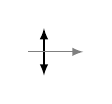
\begin{tikzpicture}
    \draw[latex-latex] (0,-.3) -- (0,+.3);
    \draw[draw=gray,-latex] (-.2,0) -- (+.5,0);
\end{tikzpicture}}}{\color{lightgray}\vert}\enspace m\uparrow^{+1}\raisebox{-.4em}{\smash{\begin{tikzpicture}
    \draw (0,0) ellipse (.8em and .3em);
    \draw[draw=gray,-latex] (0,-.3) -- (0,+.3);
    \draw[draw=gray,-latex] (-.2,0) -- (+.8,0);
    \draw[latex-latex] (.3,-.15) -- (.7,.15);
    \draw[-latex] (0,0) [partial ellipse=330:210:.8em and .3em];
\end{tikzpicture}}} &&
    \end{flalign*}
\end{cheatresume}
\columnbreak
\newheader{\bili{}{二原子分子}}
\begin{cheatresume}
$\begin{array}{@{}c!{\color{lightgray}\vrule}c}
        \+:c1{@{}l!{\color{lightgray}\vrule}}{\mathitem{準位}\ E\+_e_ + E\+_v_ + E\+_r_} & \+:r4{$\begin{array}{@{}l}
            \displaystyle E\+_v_ = \brac{\pare{v + \half} - \eta\pare{v + \half}^2} \epsilon \\
            v \downarrow 0: \tilde{\nu} = v\tilde{\nu}_0 - v\pare{v+1}\eta \tilde{\nu}_0 \\
            \displaystyle \epsilon = h\nu_0,\quad \nu_0 = 1/\pare{2\pi}\sqrt{{k}/{\mu}}
        \end{array}$} \\
        \displaystyle E\+_r_ = \pare{{\hbar^2}/{2I}}J\pare{J+1} &  \\
        J\downarrow_{-1}: \tilde{\nu}_J = 2BJ &  \\
        \displaystyle I = \mu R_0^2,\ B = {\hbar}/{4\pi Ic} & 
\end{array}$\newline
\begin{tabular}{@{}l!{\color{lightgray}\vrule}l}
    \mathitem{$\Delta n\+_e_ = 0$の場合} & \mathitem{電子と分子の角運動量} \\
    \mathitem{(振動回転スペクトル)} & \+:r3{\parbox{3.75cm}{\begin{flalign*}
        & l_z = m_l\begin{cases}
            \sigma, l_z=0 \\
            \pi,\cdots, l_z = \pm l
        \end{cases} \\
        & M_L = \sum m_l, \Lambda = \abs{M_L} \\
        & \Sigma = S,S-1,\cdots,-S \\
        & \Omega = \abs{\Lambda + \Sigma}
    \end{flalign*}\\[-2.5em]\begin{tikzpicture}[yscale=0.6]
        \draw (0,0) -- (.5,0) node[midway, above] {$^3\Delta$};
        \draw (1,0) -- (1.5,0) node[right] {$^3\Delta_1$};
        \draw (1,0.5) -- (1.5,.5) node[right] {$^3\Delta_2$};
        \draw (1,1) -- (1.5,1) node[right] {$^3\Delta_3$};
        \draw[dashed,lightgray] (.5,0) -- (1,0) (.5,0) -- (1,.5) (.5,0) -- (1,1);
        \draw[dashed,lightgray] (1.5,.5) -- (2.25,.5) (2.25,.5) -- (2.5,.75) (2.25,.5) -- (2.5,.25);
        \draw (2.5,.75) -- (3,.75) node[right]{$+\Lambda$};
        \draw (2.5,.25) -- (3,.25) node[right]{$-\Lambda$};
        \draw (1.25,0) node[below] {\scriptsize\color{lightgray}スピン軌道項};
        \draw (2.75,.25) node[below] {\scriptsize\color{lightgray}Zeeman};
    \end{tikzpicture} } } \\
    \mathitem{(赤外吸収)} & \\
    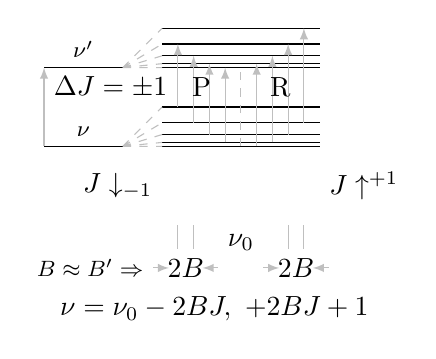
\begin{tikzpicture}
        \draw (0,0) -- (1,0) node[midway, above] {\footnotesize$\nu$};
        \draw (1.5,0) -- (3.5,0);
        \draw (1.5,0.05) -- (3.5,0.05);
        \draw (1.5,0.15) -- (3.5,0.15);
        \draw (1.5,0.3) -- (3.5,0.3);
        \draw (1.5,0.5) -- (3.5,0.5);
        \draw[dashed, lightgray] (1,0) -- (1.5,0)
        (1,0) -- (1.5,0.05)
        (1,0) -- (1.5,0.15)
        (1,0) -- (1.5,0.3)
        (1,0) -- (1.5,0.5);
        \draw (0,1) -- (1,1) node[midway, above] {\footnotesize$\nu'$};
        \draw (1.5,1) -- (3.5,1);
        \draw (1.5,1.05) -- (3.5,1.05);
        \draw (1.5,1.15) -- (3.5,1.15);
        \draw (1.5,1.3) -- (3.5,1.3);
        \draw (1.5,1.5) -- (3.5,1.5);
        \draw[dashed, lightgray] (1,1) -- (1.5,1)
        (1,1) -- (1.5,1.05)
        (1,1) -- (1.5,1.15)
        (1,1) -- (1.5,1.3)
        (1,1) -- (1.5,1.5);
        \draw[latex-, lightgray] (0.0,1) -- (0.0,0);
        \draw (0.0,0.75) node[right] {$\Delta J = \pm 1$};
        %
        \draw[-latex,lightgray]
        (1.7,0.5) -- (1.7,1.3);
        \draw[-latex,lightgray]
        (1.9,0.3) -- (1.9,1.15);
        \draw[-latex,lightgray]
        (2.1,0.15) -- (2.1,1.05);
        \draw[-latex,lightgray]
        (2.3,0.05) -- (2.3,1);
        \draw[-latex,lightgray]
        (2.7,0) -- (2.7,1.05);
        \draw[-latex,lightgray]
        (2.9,0.05) -- (2.9,1.15);
        \draw[-latex,lightgray]
        (3.1,0.15) -- (3.1,1.3);
        \draw[-latex,lightgray]
        (3.3,0.3) -- (3.3,1.5)
        ;
        \draw[dashed,lightgray] (2.5,0) -- (2.5,1);
        \draw (2.0,0.75) node {P};
        \draw (3.0,0.75) node {R};
        \draw[domain=1.6:3.4,samples=200] plot[id=comb] function { 0.1*0.25 * (atan(10*(x-2.5)))**2 * sin(0.8*3.14159*sqrt(abs(x-2.5)))**2 * (1/( sin(5*pi*(x-2.5))**2 + 0.05 ) - 1/1.05) - 1 };
        \draw[domain=1.5:3.5] plot function { -1 };
        \draw (1.5,-0.5) node[left] {$J\downarrow_{-1}$};
        \draw (3.5,-0.5) node[right] {$J\uparrow^{+1}$};
        \draw (2.5,-1) node[below] {$\nu_0$};
        \draw[lightgray] (3.1,-1) -- (3.1,-1.3);
        \draw[lightgray] (3.3,-1) -- (3.3,-1.3);
        \draw (3.2,-1.3) node[below] (2Bright) {$\kern-4pt\relax2B\kern-4pt\relax$};
        \draw[lightgray] (1.7,-1) -- (1.7,-1.3);
        \draw[lightgray] (1.9,-1) -- (1.9,-1.3);
        \draw (1.8,-1.3) node[below] (2Bleft) {$\kern-4pt\relax2B\kern-4pt\relax$};
        \node[below right = 0em and -5.5em of 2Bleft] {$\nu = \nu_0-2BJ,\ + 2B\pare{J+1} $};
        \draw[latex-,lightgray] (2Bleft.west) --++ (-0.2,0) node (2BLeftArrowLeft) {};
        \draw[latex-,lightgray] (2Bleft.east) --++ (0.2,0);
        \draw[latex-,lightgray] (2Bright.west) --++ (-0.2,0);
        \draw[latex-,lightgray] (2Bright.east) --++ (0.2,0);
        \draw (2BLeftArrowLeft) node[left] {\footnotesize $B\approx B' \Rightarrow $};
    \end{tikzpicture} &
\end{tabular}\newline
\mathitem{$LS$結合\wdiv Slaterダイアグラム}\\
\resizebox{\hsize}{!}{$ \underbrace{\begin{array}{c|ccc}
    &   & M_S & \\
    \hline
    &   & 1   & \\
M_L & 1 & 2   & 1\\
    &   & 1   & 
\end{array}}_{\displaystyle \pare{\pi\+_u_\mathrm{2p}}^2} = \underbrace{\begin{array}{c|ccc}
    &   & M_S & \\
    \hline
    &   &     & \\
M_L & 1 & 1   & 1\\
    &   &     & 
\end{array}}_{\displaystyle \Lambda = 0, S = 1\Rightarrow {^3\Sigma}} + 
\underbrace{\begin{array}{c|ccc}
    &   & M_S & \\
    \hline
    &   & 1   & \\
M_L &   &     & \\
    &   & 1   & 
\end{array}}_{\displaystyle \Lambda = 2, S = 0\Rightarrow {^1\Delta}} + 
\underbrace{\begin{array}{c|ccc}
    &   & M_S & \\
    \hline
    &   &     & \\
M_L &   & 1   & \\
    &   &     & 
\end{array}}_{\displaystyle \Lambda = 0, S = 0\Rightarrow {^1\Sigma}} $} \\[.5em]
\mathitem{$\Delta n\+_e_ \neq 0$の場合(電子振動回転スペクトル)}
\begin{tabular}{@{}c@{}c}
    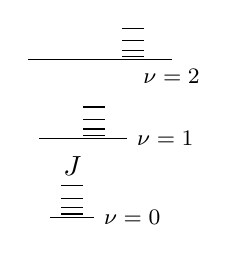
\begin{tikzpicture}[xscale=0.7]
        \draw[domain=0.37:3] plot function {(1/(9*x*x)-1/(3*x))*20+5};
        \draw (0.4,0.5) -- (1.2,0.5) node[right] {\footnotesize$\nu = 0$};
        \draw (0.6,0.54) -- (1,0.54);
        \draw (0.6,0.62) -- (1,0.62);
        \draw (0.6,0.74) -- (1,0.74);
        \draw (0.6,0.9) -- (1,0.9) node[midway,above] {$J$};
        \draw (0.2,1.5) -- (1.8,1.5) node[right] {\footnotesize$\nu = 1$};
        \draw (1.0,1.54) -- (1.4,1.54);
        \draw (1.0,1.62) -- (1.4,1.62);
        \draw (1.0,1.74) -- (1.4,1.74);
        \draw (1.0,1.9) -- (1.4,1.9);
        \draw (0.0,2.5) -- (2.6,2.5) node[below] {\footnotesize$\nu = 2$};
        \draw (1.7,2.54) -- (2.1,2.54);
        \draw (1.7,2.62) -- (2.1,2.62);
        \draw (1.7,2.74) -- (2.1,2.74);
        \draw (1.7,2.9) -- (2.1,2.9);
    \end{tikzpicture} &
    \def\rotlevel#1#2{\draw (2,#1) -- (8.25,#1) node[right] (level#1#2) {\footnotesize $#2$}}
    \def\transition#1#2#3{\draw[-latex,lightgray] (#1,#2) -- (#1,#3)}
    \def\uptransition#1#2#3{\draw[-latex] (#1,#2) -- (#1,#3)}
    \def\downtransition#1#2#3{\draw[-latex] (#1,#2) -- (#1,#3)}
    \begin{tikzpicture}[xscale=0.8,yscale=0.4]
        \draw[dashed] (1,0.25) -- (2,0.25) node[above left] {$^3{\Pi}\+_u_$};
        \draw[dashed] (1,5.25) -- (2,5.25) node[above left] {$^3{\Pi}\+_g_$};
        \rotlevel{0.5}{0};
        \rotlevel{1}{1};
        \rotlevel{1.5}{2};
        \rotlevel{2}{3};
        \rotlevel{2.5}{4};
        \rotlevel{3}{5};
        %
        \rotlevel{5.5}{0};
        \rotlevel{6}{1};
        \rotlevel{6.5}{2};
        \rotlevel{7}{3};
        \rotlevel{7.5}{4};
        \rotlevel{8}{5};
        %
        \draw (level85) node[above] {\footnotesize $\nu$};
        %
        \transition{2.15}{7}{3};
        \transition{2.3}{6.5}{2.5};
        \transition{2.45}{6}{2};
        \transition{2.6}{5.5}{1.5};
        \draw (2.375,8) -- (2.375,8) node[midway,above] {\footnotesize $\pare{0,2}$};
        %
        \transition{2.9}{7.5}{3};
        \transition{3.05}{7}{2.5};
        \transition{3.2}{6.5}{2};
        \transition{3.35}{6}{1.5};
        \transition{3.5}{5.5}{1};
        \draw (3.2,8) -- (3.2,8) node[midway,above] {\footnotesize $\pare{0,1}$};
        %
        \transition{3.8}{6.5}{1.5};
        \transition{3.95}{6}{1};
        \transition{4.1}{5.5}{0.5};
        \draw (3.95,8) -- (3.95,8) node[midway,above] {\footnotesize $\pare{0,0}$};
        %
        \transition{4.4}{8}{2.5};
        \transition{4.55}{7.5}{2};
        \transition{4.7}{7}{1.5};
        \transition{4.85}{6.5}{1};
        \transition{5}{6}{0.5};
        \draw (4.7,8) -- (4.7,8) node[midway,above] {\footnotesize $\pare{1,0}$};
        %
        \transition{5.3}{7.5}{1.5};
        \transition{5.45}{7}{1};
        \transition{5.6}{6.5}{0.5};
        \draw (5.45,8) -- (5.45,8) node[midway,above] (rightMostIndex) {\footnotesize $\pare{2,0}$};
        \draw (rightMostIndex) node[right,anchor=west] {\footnotesize \quad\color{lightgray} $\leftarrow$ Index};
        %
        \draw[dashed,-latex] (1.8,5) -- (1.8,0);
        %
        % Raman
        \uptransition{6.3}{0.5}{7};
        \downtransition{6.6}{7}{1};
        \draw[draw=none] (6.6,5.5) -- (6.6,3) node[midway, above, sloped]{\color{lightgray}\footnotesize Stokes};
        %
        \uptransition{7.3}{1}{7};
        \downtransition{7.6}{7}{0.5};
        \draw[draw=none] (7.6,5.5) -- (7.6,3) node[midway, above, sloped]{\color{lightgray}\footnotesize \stackanchor{Anti-}{Stokes}};
    \end{tikzpicture} \\[-1em]
    \scriptsize\color{lightgray}{エネルギー準位} & \scriptsize\color{lightgray}{振動スペクトル}
\end{tabular}\\[-.5em]
\begin{tabular}{@{}cc}
    \begin{tikzpicture}[xscale=1,baseline={(current bounding box.north)},outer sep=0pt,inner sep=0pt]
        \draw (0,0) -- (1,0) node[midway, above] {\footnotesize$\nu$};
        \draw (1.5,0) -- (4.5,0);
        \draw (1.5,0.05) -- (4.5,0.05);
        \draw (1.5,0.15) -- (4.5,0.15);
        \draw (1.5,0.3) -- (4.5,0.3);
        \draw (1.5,0.5) -- (4.5,0.5);
        \draw[dashed, lightgray] (1,0) -- (1.5,0)
        (1,0) -- (1.5,0.05)
        (1,0) -- (1.5,0.15)
        (1,0) -- (1.5,0.3)
        (1,0) -- (1.5,0.5);
        \draw (0,1) -- (1,1) node[midway, above] {\footnotesize$\nu'$};
        \draw (1.5,1) -- (4.5,1);
        \draw (1.5,1.05) -- (4.5,1.05);
        \draw (1.5,1.15) -- (4.5,1.15);
        \draw (1.5,1.3) -- (4.5,1.3);
        \draw (1.5,1.5) -- (4.5,1.5);
        \draw[dashed, lightgray] (1,1) -- (1.5,1)
        (1,1) -- (1.5,1.05)
        (1,1) -- (1.5,1.15)
        (1,1) -- (1.5,1.3)
        (1,1) -- (1.5,1.5);
        \draw[latex-, lightgray] (0.0,1) -- (0.0,0);
        \draw (0.0,0.75) node[right] {$\Delta J = \text{\stackanchor{$0,$}{$\pm 1$}}$};
        %
        \draw[-latex,lightgray]
        (1.7,0.5) -- (1.7,1.3);
        \draw[-latex,lightgray]
        (1.9,0.3) -- (1.9,1.15);
        \draw[-latex,lightgray]
        (2.1,0.15) -- (2.1,1.05);
        \draw[-latex,lightgray]
        (2.3,0.05) -- (2.3,1);
        \draw[-latex,lightgray]
        (2.7,0.05) -- (2.7,1.05);
        \draw[-latex,lightgray]
        (2.9,0.15) -- (2.9,1.15);
        \draw[-latex,lightgray]
        (3.1,0.3) -- (3.1,1.3);
        \draw[-latex,lightgray]
        (3.3,0.5) -- (3.3,1.5);
        \draw[-latex,lightgray]
        (3.7,0) -- (3.7,1.05);
        \draw[-latex,lightgray]
        (3.9,0.05) -- (3.9,1.15);
        \draw[-latex,lightgray]
        (4.1,0.15) -- (4.1,1.3);
        \draw[-latex,lightgray]
        (4.3,0.3) -- (4.3,1.5)
        ;

        \draw (2.0,0.75) node {P};
        \draw (3.0,0.75) node {Q};
        \draw (4.0,0.75) node {R};
        \draw (3,0) node[above] {$J=0\not\leftrightarrow 0$};
        \draw (2.25,0) node[below=.5em] {$^1\mathrm{\Sigma} \rightarrow ^1\mathrm{\Sigma}$\text{\color{lightgray}の場合には}$\Delta J \neq 0$};
    \end{tikzpicture} & \+:r1{\parbox{3.5cm}{
    \begin{align*}
        \tilde{\nu}_P &= -\pare{B'+B}J + \delta \\
        \tilde{\nu}_Q &= \pare{B'-B}J + \delta  \\
        \tilde{\nu}_R &= 2B' + \pare{3B' - B} + \delta  \\
        \delta &= \pare{B'-B}J^2
    \end{align*}
    }}
\end{tabular}\\[.5em]
\mathitem{Raman散乱}\quad $\Delta J = 0,\pm 2$\newline
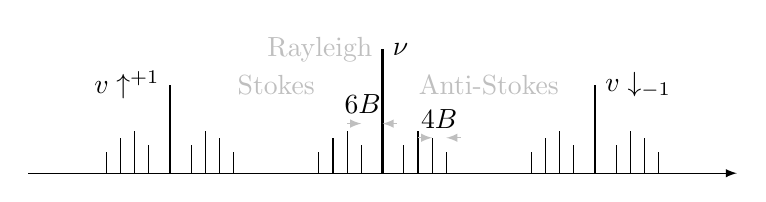
\begin{tikzpicture}[scale=0.45]
    \draw[-latex] (-10,0) -- (10,0);
    \draw[thick] (0,0) -- (0,3.5) node[left] {\color{lightgray}Rayleigh} node[right] {$\nu$};
    \draw[thick] (6,0) -- (6,2.5) node[right] {$v\downarrow_{-1}$};
    \draw (3,2.5) node {\color{lightgray} Anti-Stokes};
    \draw[thick] (-6,0) -- (-6,2.5) node[left] {$v\uparrow^{+1}$};
    \draw (-3,2.5) node {\color{lightgray} Stokes};
    \draw (0.6,0) -- (0.6,0.8);
    \draw (1,0) -- (1,1.2);
    \draw (1.4,0) -- (1.4,1);
    \draw (1.8,0) -- (1.8,0.6);
    \draw (-0.6,0) -- (-0.6,0.8);
    \draw (-1,0) -- (-1,1.2);
    \draw (-1.4,0) -- (-1.4,1);
    \draw (-1.8,0) -- (-1.8,0.6);
    \draw[-latex,lightgray] (-1,1.4) -- (-0.6,1.4);
    \draw[-latex,lightgray] (0.4,1.4) -- (0,1.4);
    \draw (-0.3,1.4) node[above] {$6B\ \ $};
    \draw[-latex,lightgray] (1,1) -- (1.4,1);
    \draw[-latex,lightgray] (2.2,1) -- (1.8,1);
    \draw (1.6,1) node[above] {$4B$};
    %
    \draw (6.6,0) -- (6.6,0.8);
    \draw (7,0) -- (7,1.2);
    \draw (7.4,0) -- (7.4,1);
    \draw (7.8,0) -- (7.8,0.6);
    \draw (5.4,0) -- (5.4,0.8);
    \draw (5,0) -- (5,1.2);
    \draw (4.6,0) -- (4.6,1);
    \draw (4.2,0) -- (4.2,0.6);
    %
    \draw (-6.6,0) -- (-6.6,0.8);
    \draw (-7,0) -- (-7,1.2);
    \draw (-7.4,0) -- (-7.4,1);
    \draw (-7.8,0) -- (-7.8,0.6);
    \draw (-5.4,0) -- (-5.4,0.8);
    \draw (-5,0) -- (-5,1.2);
    \draw (-4.6,0) -- (-4.6,1);
    \draw (-4.2,0) -- (-4.2,0.6);
\end{tikzpicture}
\end{cheatresume}

\end{multicols*}

\end{document}
